% Created by tikzDevice version 0.12.3.1 on 2021-02-28 16:46:13
% !TEX encoding = UTF-8 Unicode
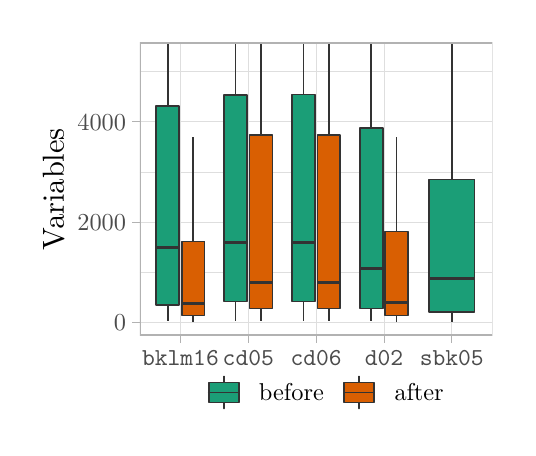
\begin{tikzpicture}[x=1pt,y=1pt]
\definecolor{fillColor}{RGB}{255,255,255}
\path[use as bounding box,fill=fillColor,fill opacity=0.00] (0,0) rectangle (173.45,144.54);
\begin{scope}
\path[clip] (  0.00,  0.00) rectangle (173.45,144.54);
\definecolor{drawColor}{RGB}{255,255,255}
\definecolor{fillColor}{RGB}{255,255,255}

\path[draw=drawColor,line width= 0.6pt,line join=round,line cap=round,fill=fillColor] (  0.00,  0.00) rectangle (173.45,144.54);
\end{scope}
\begin{scope}
\path[clip] ( 40.51, 33.38) rectangle (167.95,139.04);
\definecolor{fillColor}{RGB}{255,255,255}

\path[fill=fillColor] ( 40.51, 33.38) rectangle (167.95,139.04);
\definecolor{drawColor}{gray}{0.87}

\path[draw=drawColor,line width= 0.1pt,line join=round] ( 40.51, 56.14) --
	(167.95, 56.14);

\path[draw=drawColor,line width= 0.1pt,line join=round] ( 40.51, 92.43) --
	(167.95, 92.43);

\path[draw=drawColor,line width= 0.1pt,line join=round] ( 40.51,128.72) --
	(167.95,128.72);

\path[draw=drawColor,line width= 0.3pt,line join=round] ( 40.51, 38.00) --
	(167.95, 38.00);

\path[draw=drawColor,line width= 0.3pt,line join=round] ( 40.51, 74.29) --
	(167.95, 74.29);

\path[draw=drawColor,line width= 0.3pt,line join=round] ( 40.51,110.58) --
	(167.95,110.58);

\path[draw=drawColor,line width= 0.3pt,line join=round] ( 55.21, 33.38) --
	( 55.21,139.04);

\path[draw=drawColor,line width= 0.3pt,line join=round] ( 79.72, 33.38) --
	( 79.72,139.04);

\path[draw=drawColor,line width= 0.3pt,line join=round] (104.23, 33.38) --
	(104.23,139.04);

\path[draw=drawColor,line width= 0.3pt,line join=round] (128.74, 33.38) --
	(128.74,139.04);

\path[draw=drawColor,line width= 0.3pt,line join=round] (153.24, 33.38) --
	(153.24,139.04);
\definecolor{drawColor}{gray}{0.20}

\path[draw=drawColor,line width= 0.6pt,line join=round] ( 50.62,116.24) -- ( 50.62,144.54);

\path[draw=drawColor,line width= 0.6pt,line join=round] ( 50.62, 44.35) -- ( 50.62, 38.47);
\definecolor{fillColor}{RGB}{27,158,119}

\path[draw=drawColor,line width= 0.6pt,line join=round,line cap=round,fill=fillColor] ( 46.48,116.24) --
	( 46.48, 44.35) --
	( 54.75, 44.35) --
	( 54.75,116.24) --
	( 46.48,116.24) --
	cycle;

\path[draw=drawColor,line width= 1.1pt,line join=round] ( 46.48, 65.20) -- ( 54.75, 65.20);

\path[draw=drawColor,line width= 0.6pt,line join=round] ( 59.81, 67.32) -- ( 59.81,104.99);

\path[draw=drawColor,line width= 0.6pt,line join=round] ( 59.81, 40.54) -- ( 59.81, 38.18);
\definecolor{fillColor}{RGB}{217,95,2}

\path[draw=drawColor,line width= 0.6pt,line join=round,line cap=round,fill=fillColor] ( 55.67, 67.32) --
	( 55.67, 40.54) --
	( 63.95, 40.54) --
	( 63.95, 67.32) --
	( 55.67, 67.32) --
	cycle;

\path[draw=drawColor,line width= 1.1pt,line join=round] ( 55.67, 44.82) -- ( 63.95, 44.82);

\path[draw=drawColor,line width= 0.6pt,line join=round] ( 75.13,120.28) -- ( 75.13,144.54);

\path[draw=drawColor,line width= 0.6pt,line join=round] ( 75.13, 45.62) -- ( 75.13, 38.58);
\definecolor{fillColor}{RGB}{27,158,119}

\path[draw=drawColor,line width= 0.6pt,line join=round,line cap=round,fill=fillColor] ( 70.99,120.28) --
	( 70.99, 45.62) --
	( 79.26, 45.62) --
	( 79.26,120.28) --
	( 70.99,120.28) --
	cycle;

\path[draw=drawColor,line width= 1.1pt,line join=round] ( 70.99, 66.74) -- ( 79.26, 66.74);

\path[draw=drawColor,line width= 0.6pt,line join=round] ( 84.32,105.79) -- ( 84.32,144.54);

\path[draw=drawColor,line width= 0.6pt,line join=round] ( 84.32, 43.08) -- ( 84.32, 38.42);
\definecolor{fillColor}{RGB}{217,95,2}

\path[draw=drawColor,line width= 0.6pt,line join=round,line cap=round,fill=fillColor] ( 80.18,105.79) --
	( 80.18, 43.08) --
	( 88.45, 43.08) --
	( 88.45,105.79) --
	( 80.18,105.79) --
	cycle;

\path[draw=drawColor,line width= 1.1pt,line join=round] ( 80.18, 52.51) -- ( 88.45, 52.51);

\path[draw=drawColor,line width= 0.6pt,line join=round] ( 99.63,120.34) -- ( 99.63,144.54);

\path[draw=drawColor,line width= 0.6pt,line join=round] ( 99.63, 45.62) -- ( 99.63, 38.58);
\definecolor{fillColor}{RGB}{27,158,119}

\path[draw=drawColor,line width= 0.6pt,line join=round,line cap=round,fill=fillColor] ( 95.50,120.34) --
	( 95.50, 45.62) --
	(103.77, 45.62) --
	(103.77,120.34) --
	( 95.50,120.34) --
	cycle;

\path[draw=drawColor,line width= 1.1pt,line join=round] ( 95.50, 66.74) -- (103.77, 66.74);

\path[draw=drawColor,line width= 0.6pt,line join=round] (108.82,105.79) -- (108.82,144.54);

\path[draw=drawColor,line width= 0.6pt,line join=round] (108.82, 43.08) -- (108.82, 38.42);
\definecolor{fillColor}{RGB}{217,95,2}

\path[draw=drawColor,line width= 0.6pt,line join=round,line cap=round,fill=fillColor] (104.69,105.79) --
	(104.69, 43.08) --
	(112.96, 43.08) --
	(112.96,105.79) --
	(104.69,105.79) --
	cycle;

\path[draw=drawColor,line width= 1.1pt,line join=round] (104.69, 52.51) -- (112.96, 52.51);

\path[draw=drawColor,line width= 0.6pt,line join=round] (124.14,108.25) -- (124.14,144.54);

\path[draw=drawColor,line width= 0.6pt,line join=round] (124.14, 43.08) -- (124.14, 38.40);
\definecolor{fillColor}{RGB}{27,158,119}

\path[draw=drawColor,line width= 0.6pt,line join=round,line cap=round,fill=fillColor] (120.01,108.25) --
	(120.01, 43.08) --
	(128.28, 43.08) --
	(128.28,108.25) --
	(120.01,108.25) --
	cycle;

\path[draw=drawColor,line width= 1.1pt,line join=round] (120.01, 57.40) -- (128.28, 57.40);

\path[draw=drawColor,line width= 0.6pt,line join=round] (133.33, 70.91) -- (133.33,104.99);

\path[draw=drawColor,line width= 0.6pt,line join=round] (133.33, 40.54) -- (133.33, 38.18);
\definecolor{fillColor}{RGB}{217,95,2}

\path[draw=drawColor,line width= 0.6pt,line join=round,line cap=round,fill=fillColor] (129.20, 70.91) --
	(129.20, 40.54) --
	(137.47, 40.54) --
	(137.47, 70.91) --
	(129.20, 70.91) --
	cycle;

\path[draw=drawColor,line width= 1.1pt,line join=round] (129.20, 45.26) -- (137.47, 45.26);

\path[draw=drawColor,line width= 0.6pt,line join=round] (153.24, 89.69) -- (153.24,144.54);

\path[draw=drawColor,line width= 0.6pt,line join=round] (153.24, 41.81) -- (153.24, 38.29);
\definecolor{fillColor}{RGB}{27,158,119}

\path[draw=drawColor,line width= 0.6pt,line join=round,line cap=round,fill=fillColor] (144.97, 89.69) --
	(144.97, 41.81) --
	(161.51, 41.81) --
	(161.51, 89.69) --
	(144.97, 89.69) --
	cycle;

\path[draw=drawColor,line width= 1.1pt,line join=round] (144.97, 53.85) -- (161.51, 53.85);
\definecolor{drawColor}{gray}{0.70}

\path[draw=drawColor,line width= 0.6pt,line join=round,line cap=round] ( 40.51, 33.38) rectangle (167.95,139.04);
\end{scope}
\begin{scope}
\path[clip] (  0.00,  0.00) rectangle (173.45,144.54);
\definecolor{drawColor}{gray}{0.30}

\node[text=drawColor,anchor=base east,inner sep=0pt, outer sep=0pt, scale=  0.88] at ( 35.56, 34.97) {0};

\node[text=drawColor,anchor=base east,inner sep=0pt, outer sep=0pt, scale=  0.88] at ( 35.56, 71.26) {2000};

\node[text=drawColor,anchor=base east,inner sep=0pt, outer sep=0pt, scale=  0.88] at ( 35.56,107.55) {4000};
\end{scope}
\begin{scope}
\path[clip] (  0.00,  0.00) rectangle (173.45,144.54);
\definecolor{drawColor}{gray}{0.70}

\path[draw=drawColor,line width= 0.3pt,line join=round] ( 37.76, 38.00) --
	( 40.51, 38.00);

\path[draw=drawColor,line width= 0.3pt,line join=round] ( 37.76, 74.29) --
	( 40.51, 74.29);

\path[draw=drawColor,line width= 0.3pt,line join=round] ( 37.76,110.58) --
	( 40.51,110.58);
\end{scope}
\begin{scope}
\path[clip] (  0.00,  0.00) rectangle (173.45,144.54);
\definecolor{drawColor}{gray}{0.70}

\path[draw=drawColor,line width= 0.3pt,line join=round] ( 55.21, 30.63) --
	( 55.21, 33.38);

\path[draw=drawColor,line width= 0.3pt,line join=round] ( 79.72, 30.63) --
	( 79.72, 33.38);

\path[draw=drawColor,line width= 0.3pt,line join=round] (104.23, 30.63) --
	(104.23, 33.38);

\path[draw=drawColor,line width= 0.3pt,line join=round] (128.74, 30.63) --
	(128.74, 33.38);

\path[draw=drawColor,line width= 0.3pt,line join=round] (153.24, 30.63) --
	(153.24, 33.38);
\end{scope}
\begin{scope}
\path[clip] (  0.00,  0.00) rectangle (173.45,144.54);
\definecolor{drawColor}{gray}{0.30}

\node[text=drawColor,anchor=base,inner sep=0pt, outer sep=0pt, scale=  0.88] at ( 55.21, 22.37) {\texttt{bklm16}};

\node[text=drawColor,anchor=base,inner sep=0pt, outer sep=0pt, scale=  0.88] at ( 79.72, 22.37) {\texttt{cd05}};

\node[text=drawColor,anchor=base,inner sep=0pt, outer sep=0pt, scale=  0.88] at (104.23, 22.37) {\texttt{cd06}};

\node[text=drawColor,anchor=base,inner sep=0pt, outer sep=0pt, scale=  0.88] at (128.74, 22.37) {\texttt{d02}};

\node[text=drawColor,anchor=base,inner sep=0pt, outer sep=0pt, scale=  0.88] at (153.24, 22.37) {\texttt{sbk05}};
\end{scope}
\begin{scope}
\path[clip] (  0.00,  0.00) rectangle (173.45,144.54);
\definecolor{drawColor}{RGB}{0,0,0}

\node[text=drawColor,rotate= 90.00,anchor=base,inner sep=0pt, outer sep=0pt, scale=  1.10] at ( 13.08, 86.21) {Variables};
\end{scope}
\begin{scope}
\path[clip] (  0.00,  0.00) rectangle (173.45,144.54);
\definecolor{fillColor}{RGB}{255,255,255}

\path[fill=fillColor] ( 58.10,  5.50) rectangle (150.36, -2.81);
\end{scope}
\begin{scope}
\path[clip] (  0.00,  0.00) rectangle (173.45,144.54);
\definecolor{fillColor}{RGB}{255,255,255}

\path[fill=fillColor] ( 63.60,  5.50) rectangle ( 78.05, 19.95);
\end{scope}
\begin{scope}
\path[clip] (  0.00,  0.00) rectangle (173.45,144.54);
\definecolor{drawColor}{gray}{0.20}

\path[draw=drawColor,line width= 0.6pt,line join=round,line cap=round] ( 70.83,  6.95) --
	( 70.83,  9.11);

\path[draw=drawColor,line width= 0.6pt,line join=round,line cap=round] ( 70.83, 16.34) --
	( 70.83, 18.51);
\definecolor{fillColor}{RGB}{27,158,119}

\path[draw=drawColor,line width= 0.6pt,line join=round,line cap=round,fill=fillColor] ( 65.41,  9.11) rectangle ( 76.25, 16.34);

\path[draw=drawColor,line width= 0.6pt,line join=round,line cap=round] ( 65.41, 12.73) --
	( 76.25, 12.73);
\end{scope}
\begin{scope}
\path[clip] (  0.00,  0.00) rectangle (173.45,144.54);
\definecolor{fillColor}{RGB}{255,255,255}

\path[fill=fillColor] (112.54,  5.50) rectangle (126.99, 19.95);
\end{scope}
\begin{scope}
\path[clip] (  0.00,  0.00) rectangle (173.45,144.54);
\definecolor{drawColor}{gray}{0.20}

\path[draw=drawColor,line width= 0.6pt,line join=round,line cap=round] (119.77,  6.95) --
	(119.77,  9.11);

\path[draw=drawColor,line width= 0.6pt,line join=round,line cap=round] (119.77, 16.34) --
	(119.77, 18.51);
\definecolor{fillColor}{RGB}{217,95,2}

\path[draw=drawColor,line width= 0.6pt,line join=round,line cap=round,fill=fillColor] (114.35,  9.11) rectangle (125.19, 16.34);

\path[draw=drawColor,line width= 0.6pt,line join=round,line cap=round] (114.35, 12.73) --
	(125.19, 12.73);
\end{scope}
\begin{scope}
\path[clip] (  0.00,  0.00) rectangle (173.45,144.54);
\definecolor{drawColor}{RGB}{0,0,0}

\node[text=drawColor,anchor=base west,inner sep=0pt, outer sep=0pt, scale=  0.88] at ( 83.55,  9.70) {before};
\end{scope}
\begin{scope}
\path[clip] (  0.00,  0.00) rectangle (173.45,144.54);
\definecolor{drawColor}{RGB}{0,0,0}

\node[text=drawColor,anchor=base west,inner sep=0pt, outer sep=0pt, scale=  0.88] at (132.49,  9.70) {after};
\end{scope}
\end{tikzpicture}
